\let\negmedspace\undefined
\let\negthickspace\undefined
\documentclass[journal,12pt,twocolumn]{IEEEtran}
\usepackage{cite}
\usepackage{amsmath,amssymb,amsfonts,amsthm}
\usepackage{algorithmic}
\usepackage{graphicx}
\usepackage{textcomp}
\usepackage{xcolor}
\usepackage{txfonts}
\usepackage{listings}
\usepackage{enumitem}
\usepackage{mathtools}
\usepackage{gensymb}
\usepackage{comment}
\usepackage[breaklinks=true]{hyperref}
\usepackage{tkz-euclide} 
\usepackage{listings}
\usepackage{gvv}                                        
\def\inputGnumericTable{}                                 
\usepackage[latin1]{inputenc}                                
\usepackage{color}                                            
\usepackage{array}                                            
\usepackage{longtable}                                       
\usepackage{calc}                                             
\usepackage{multirow}                                         
\usepackage{hhline}                                           
\usepackage{ifthen}                                           
\usepackage{lscape}
\usepackage{caption}
\newtheorem{theorem}{Theorem}[section]
\newtheorem{problem}{Problem}
\newtheorem{proposition}{Proposition}[section]
\newtheorem{lemma}{Lemma}[section]
\newtheorem{corollary}[theorem]{Corollary}
\newtheorem{example}{Example}[section]
\newtheorem{definition}[problem]{Definition}
\newcommand{\BEQA}{\begin{eqnarray}}
\newcommand{\EEQA}{\end{eqnarray}}
\newcommand{\define}{\stackrel{\triangle}{=}}
\theoremstyle{remark}
\newtheorem{rem}{Remark}
\begin{document}

\bibliographystyle{IEEEtran}
\vspace{3cm}

\title{10.5.2.14}
\author{EE23BTECH11003 - pranav}
\maketitle
\newpage

\bigskip
\renewcommand{\thefigure}{\arabic{figure}}
\renewcommand{\thetable}{\arabic{table}}

\textbf{Question}:A spring having with a spring constant 1200 N$m^{-1}$ is mounted on a horizontal
table as shown in Fig.A mass of 3 kg is attached to the free end of the
spring. The mass is then pulled sideways to a distance of 2.0 cm and released.\\
Determine (i) the frequency of oscillations, (ii) maximum acceleration of the mass,
and (iii) the maximum speed of the mass
\begin{figure}[h!]
    \centering
    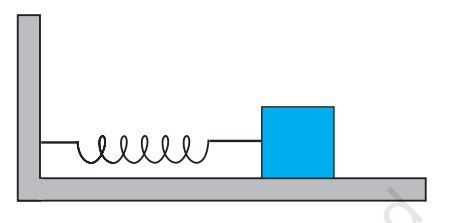
\includegraphics[width=0.5\linewidth]{figs/figure.jpg}
    \caption{ }
    
\end{figure}\\
\solution
\begin{table}[h]
    \centering
    \input{tables/Table.Tex}
    \caption{Variables Used}
    \label{tab:table_11.9.3.6}
\end{table}
at $t=0$
\begin{align}
A&=A\sin{(w(0)+\phi)}\\
\implies \phi&=\frac{\pi}{2}\\
\implies x(t)&=A\cos{wt} 
\end{align}
\begin{figure}[h!]
    \centering
    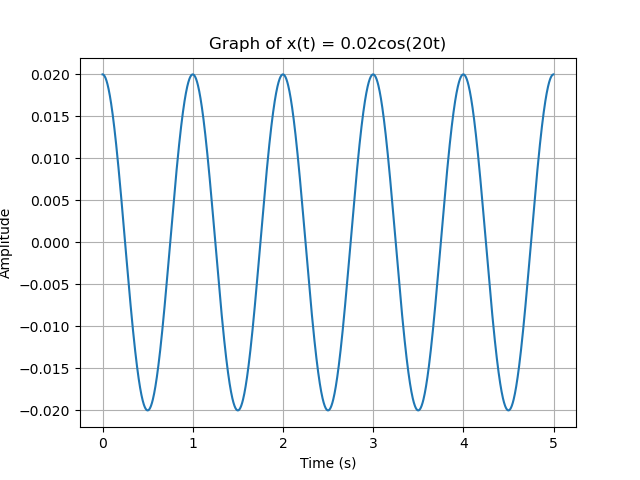
\includegraphics[width=1.1\linewidth]{figs/analog1.png}
    \caption{Enter Caption}
    \label{fig:enter-label}
\end{figure}\\
(i) frequency of the oscillation
\begin{align}
    f&=\frac{\omega}{2\pi}\\\
    \implies f&=\frac{10}{\pi}
\end{align}
(iii)maximum speed of mass\\
\begin{align}
    x(t)&=0.02\cos{20t}\\
    v(t)&=\frac{dx(t)}{dt}= -0.4\sin{20t}\\
    v_{\text{max}}&=0.4m/s    
\end{align}
\begin{figure}[h!]
    \centering
    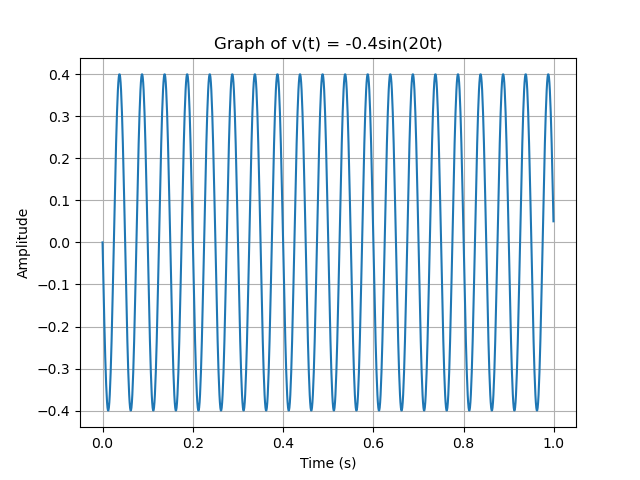
\includegraphics[width=1.1\linewidth]{figs/analog2.png}
    \caption{Enter Caption}
    \label{fig:enter-label}
\end{figure}\\
(ii)maximum accelaration of mass\\
\begin{align}
    a(t)&=\frac{dv(t)}{dt}=-8\cos{20t}\\
    a_{max}&=8m/s^{2}
\end{align}
\begin{figure}[h!]
    \centering
    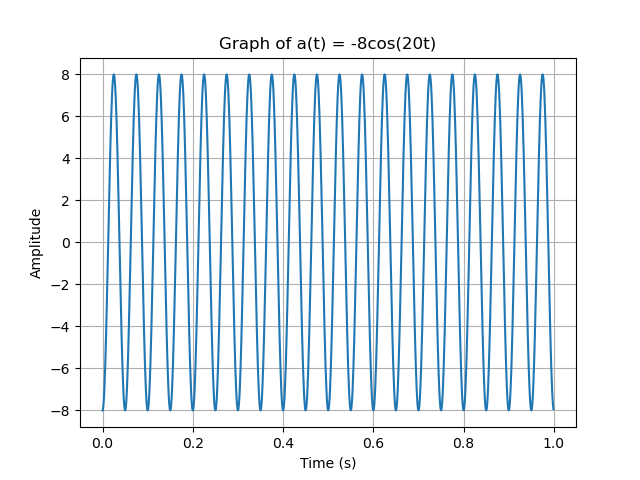
\includegraphics[width=1.1\linewidth]{figs/analog3.png}
    \caption{Enter Caption}
    \label{fig:enter-label}
\end{figure}
\end{document}
